\documentclass{article}
\usepackage{graphicx} % Required for inserting images
\usepackage[colorlinks=true, linkcolor=blue]{hyperref}

\title{Cloud Computing Project : Variant 3 — Small files problem \& compaction}
\author{Tanguy Godat \& Tim Gouvernon}
\date{April 2026}

\begin{document}

\maketitle
\iffalse
\section{TO-DO List}
Faire script Dataset\\
Générer Dataset\\
Script compaction\\
Décider si garder en local ou vm\\



\section{Questions}
Can we use os (import)\\
Is the compacted file only in terms of number of files or also "compacting" data (ie. convert string to int with a dictionary) TO BOTH \\
Order : dataset\_gen.py $\rightarrow$ compact.py $\rightarrow$ upload.py $\rightarrow$ bench.py $\rightarrow$ analysis.ipynb $\rightarrow$ download.py\\
For now total size is 5.3GB, using rows size rather than size, should we go with more line ?\\
What is Raw data for us ? NO\\
Can we get a vm with 10GB so we have 4 core and not only one (azure)\\

\section{Question: 04.05}
In end-to-end pipeline time, do we have to do the compacted version also, if yes, do we have to generate the small fill version first then use the compaction script or generate a compact version immediately (tldr: avoid unnecessary small-file step but don't use compacted.py) TROUVER TOUTES LES LIGNES DE PARQUET\\
Current usage of minio (s3) on the vm
Show on
(After 18.05)
yaml instead of too many parameter in parser
run multiple time for accurate value (Medium set for listing has intriguing value value)
for the visual, after each step (generation, compaction, upload, listing,... ) append value in csv or temp list in order to update visual graph instead of appending the whole at the end
\fi
\section{Chosen Variant \& Methodology}

\subsection{Chosen Variant}
After reviewing the proposed project variants, we selected variant 3, which focuses on small files and compaction. This variant was considered the most relevant because it addresses a practical performance issue that can also be observed in everyday computer usage: handling many small files is often less efficient than handling fewer large files. Based on this intuition, the initial hypothesis was that workloads composed of many small files would require more processing time than equivalent workloads with larger files, with an expected slowdown on the order of a factor of three.

\subsection{Methodology}
The work was organized around a MinIO-based storage environment deployed in Docker, which provided a reproducible setup for testing file ingestion and retrieval. The first step was to prepare the dataset generator and the compaction script, since these two components defined the workloads that would later be benchmarked.

Once the test data had been generated, the datasets were uploaded to MinIO and then downloaded again in order to measure the impact of file size and file count on storage performance. This allowed the comparison of small-file workloads with compacted workloads under the same experimental conditions.

To evaluate the system consistently, benchmark runs were repeated for the different dataset scales S, M, and L having respectively 5M, 25M and 100M rows. The benchmark results were collected for both upload and download operations, making it possible to compare performance before and after compaction and to observe how the effect evolved with dataset size.

All experiments were performed in a controlled Docker environment to reduce variability and improve reproducibility. This setup also made it easier to rerun the tests, isolate the storage component, and compare results across multiple trials.
\section{Work Repartition}

A large part of the implementation was carried out collaboratively during live vocal sessions on Discord. In practice, most development followed a pair-programming approach: both team members discussed the design choices, reviewed the code together, and contributed to the implementation, even when the final commit was made from a single account. As a result, commit authorship does not always fully reflect the actual contribution to each script.

To make the repartition clearer, the following list indicates the main responsibility areas of each team member, that is, the components for which each person contributed the most.

\paragraph{Tanguy Godat}
\begin{itemize}
    \item \texttt{bench.py}
    \item \texttt{upload.py}
    \item \texttt{download.py}
\end{itemize}

\paragraph{Tim Gouvernon}
\begin{itemize}
    \item Docker and MinIO setup and handling
    \item \texttt{dataset\_gen.py}
    \item \texttt{compaction.py}
    \item \texttt{analysis.ipynb}
\end{itemize}

Although the tasks above were divided by main area of responsibility, the project remained highly collaborative throughout its development. The implementation choices, debugging, and validation of results were discussed jointly, which means that both team members contributed to the overall design and execution of the project.

\section{Experimental results}

We evaluate Variant 3 on the S, M, and L datasets, comparing the small-files layout against the compact layout. The benchmark records upload throughput, download throughput, listing time, query time, and the number of objects for each layout.

\subsection{Setup}

The synthetic dataset uses the fixed schema required by the assignment, with \textit{ts}, \textit{user\_id}, \textit{region}, \textit{event\_type}, and \textit{value}. The benchmark runs the same filter-and-aggregate query for every size: \textit{region = tollgate\_a1\_geneva}, a fixed time window from \textit{2025-01-15} to \textit{2025-02-15}, then group by \textit{event\_type} with count and average \textit{value}.

The layout small in which each Parquet object contains 10'000 rows. The compact layout, which rewrites the same data into fewer larger files for each Parquet object contains 250'000 rows. The recorded results are in results.csv, which includes file counts, bytes transferred, listing time, query time, and end-to-end generation and compaction times.

\subsection{Summary table}

\begin{table}[h]
\centering
\footnotesize
\begin{tabular}{lllllll}
\hline
Size & Layout & Objects & Upload s & Listing s & Query s & Download s \\
\hline
S & small & 500 & 12.63 & 0.13 & 1.60 & 9.07 \\
S & compact & 20 & 3.35 & 0.02 & 0.37 & 0.67 \\
M & small & 2500 & 64.49 & 0.65 & 7.10 & 47.85 \\
M & compact & 100 & 16.64 & 0.03 & 1.79 & 4.66 \\
L & small & 10000 & 252.58 & 2.49 & 30.58 & 195.98 \\
L & compact & 400 & 63.93 & 0.16 & 6.31 & 16.63 \\
\hline
\end{tabular}
\caption{Benchmark results. Times are in seconds.}
\label{table_benchmark}
\end{table}

\begin{table}[htbp]
    \centering
    \footnotesize
    \begin{tabular}{lrrrr}
        \hline
        Size & Query speedup & Listing speedup & Download speedup & Upload speedup \\
        \hline
        S & 4.35 & 8.27 & 13.40 & 3.72 \\
        M & 3.97 & 21.01 & 10.13 & 3.82 \\
        L & 4.84 & 15.23 & 11.62 & 3.90 \\
        \hline
    \end{tabular}
    \caption{Benchmark speedup factors across dataset sizes.}
    \label{table_speedup}
\end{table}

\begin{table}[htbp]
    \centering
    \footnotesize
    \begin{tabular}{lrrrr}
        \hline
        Size & Query t.r.\ (\%) & Listing t.r.\ (\%) & Upload gain (\%) & Download gain (\%) \\
        \hline
        S & 77.04 & 87.91 & 271.56 & 1240.37 \\
        M & 74.83 & 95.24 & 282.18 & 912.93 \\
        L & 79.35 & 93.43 & 289.63 & 1062.06 \\
        \hline
    \end{tabular}
    \caption{Benchmark percentage reductions and gains across dataset sizes.}
    \label{table_reduction}
    \vspace{2mm}
    
    \begin{minipage}{0.9\linewidth}
        \footnotesize
        \textit{Note:} t.r. denotes time reduction.
    \end{minipage}
\end{table}


Overall, the results confirm that compaction significantly improves performance for all dataset sizes. By reducing the object count from 500/2500/10000 to 20/100/400 respectively, the compact layout removes much of the metadata and listing overhead associated with small files. As a result, both query and listing times decrease substantially, while upload and download throughput increase consistently. The effect is strongest on the largest dataset, where the small-files layout incurs the highest overhead. These findings support the conclusion that Variant 3 benefits strongly from file compaction.
\newpage

\section{Interpretation}
The results provide strong evidence that Variant 3 benefits substantially from compaction, and that the main source of improvement is the reduction in object count. Across all three dataset sizes, the compact layout keeps the same underlying data and query logic, but reorganizes it into far fewer files, which reduces metadata overhead and makes each operation more efficient. This is exactly the kind of workload where small-file costs become visible, because the system spends less time managing file boundaries and more time doing useful work.

A clear pattern appears in the summary table \ref{table_benchmark} : every operation becomes faster under the compact layout, and the gains remain consistent as the dataset grows. On the smallest dataset, the differences are already noticeable, but the impact becomes much more important on M and especially on L, where the small-files layout has to manage 10'000 objects. For L, query time falls from 30.58 s to 6.31 s, listing time drops from 2.49 s to 0.16 s, and download time decreases from 195.98 s to 16.63 s. These are not minor improvements; they show that the compact layout changes the overall cost profile of the benchmark.

The speedup table \ref{table_speedup} confirms that compaction helps both I/O-bound and metadata-heavy operations. Listing benefits the most, which is expected because listing many small objects is expensive and scales poorly with object count. Query speed also improves by about 4x to 5x, showing that even the analytical workload gains from a cleaner physical layout. Upload speed improves as well, though the gain is smaller than for listing or download, which suggests that upload is less sensitive to the same metadata overhead, but still benefits from fewer objects and better batching.

The reduction table \ref{table_reduction} tells the same story from the opposite perspective. Query time is reduced by roughly 75\% to 79\%, listing time by about 88\% to 95\%, and the throughput gains for upload and download are very large. The especially large download gain indicates that the compact layout is much more efficient at moving larger contiguous files than many small ones. In practice, this means the system is not just slightly better after compaction; it is operating in a different performance regime.

The figure \ref{fig:variant3-results} makes the trend easy to see visually. For every dataset size, the compact bars are much lower for request and listing time, while the throughput bars are much higher. The shape of the chart also suggests that the compact layout scales more gracefully, because performance stays relatively stable across S, M, and L compared with the small-files layout, which becomes increasingly expensive as object count rises. That is an important practical result, since scaling behavior matters more than isolated measurements in real data pipelines.

Overall, Variant 3 shows that compaction is an effective and necessary optimization when dealing with object storage at scale. The benchmark demonstrates that fewer, larger objects substantially reduce overhead and improve both latency and throughput across all tested sizes. In other words, the compact layout preserves the same data and query semantics while delivering a much better execution profile, making it the preferable strategy for this workload.

\section{Recommendation}

Based on the benchmark results, the compact layout should be preferred over the small-files layout for this workload. It consistently reduces the number of objects, which lowers metadata overhead and improves performance across all measured operations. This benefit is visible in the results for S, M, and L, where compaction improves query time, listing time, upload throughput, and download throughput in a stable and repeatable way.

The most important recommendation is to avoid producing very small files in the first place. In this benchmark, the small-files layout stores 10'000 rows per object, while the compact layout rewrites the same data into larger objects containing 250'000 rows each. This change leads to much better overall efficiency, especially as the dataset grows, because the cost of listing and managing many objects increases rapidly with scale.

For a real deployment, compaction should be applied regularly rather than only as a one-time cleanup step. A practical strategy is to write small files during ingestion if necessary, but then merge them into larger objects before repeated queries or downstream processing. This keeps ingestion flexible while preserving good query performance and reducing the overhead of object storage operations.

The benchmark also suggests that compaction is most valuable when the workload involves repeated listing, querying, or downloading of the same data. In such cases, the cost of many small objects quickly dominates execution time. Therefore, if the goal is to optimize analytical performance on object storage, the compact layout is the better choice and should be used as the default organization strategy.

Overall, Variant 3 shows that file layout has a major impact on system efficiency. The compact layout offers a clear trade-off in favor of fewer, larger objects, and the results show that this trade-off is beneficial for both latency and throughput. For this reason, compaction is the recommended approach for the benchmarked pipeline.

\section{Limitations \& threats to validity}

This evaluation has several limitations that should be kept in mind when interpreting the results. First, the benchmark was run on a single environment and therefore reflects the performance characteristics of that specific setup rather than a broader deployment population. Factors such as network quality, storage backend behavior, CPU load, and local caching can all influence the measured times, so the absolute values may not generalize directly to other systems.

A second limitation is that the benchmark uses synthetic data with a fixed schema and a controlled query pattern. While this is useful for making the comparison between the small-files and compact layouts clear, it does not capture the full diversity of real workloads. In practice, real datasets may contain different value distributions, skewed access patterns, or more complex queries, which could change the relative benefit of compaction.

Another threat to validity comes from measurement noise. Upload, download, listing, and query times can vary from run to run due to transient system activity, background processes, or temporary network fluctuations. Although the results show a consistent trend across all dataset sizes, the benchmark would be stronger if each experiment were repeated several times and summarized using averages or confidence intervals.

There is also a construct validity concern related to the choice of compaction ratio. The compact layout rewrites the data into larger objects containing 250'000 rows each, while the small-files layout uses 10'000 rows per object. This setup demonstrates the effect of compaction clearly, but different compaction thresholds could lead to different trade-offs between file size, parallelism, and overhead. As a result, the reported numbers should be understood as evidence for this particular configuration rather than as an optimal universal setting.

Finally, the benchmark focuses on a limited set of operations: upload, listing, download, and a single filter-and-aggregate query. These operations are relevant to the assignment and sufficient to show the impact of object count, but they do not cover every possible workload. More complex analytical queries, concurrent access patterns, or update-heavy workflows might produce different outcomes. Even with these limitations, the results still provide strong evidence that reducing object count improves performance in this benchmarked pipeline.
\section{Additional notes}
Why we didn't use Yaml
Why we have some weird medium value
\newpage
\pagenumbering{roman}
\setcounter{page}{1}
\section*{Graphs}
\begin{figure}[htbp]
    \centering
    \makebox[\linewidth][c]{%
        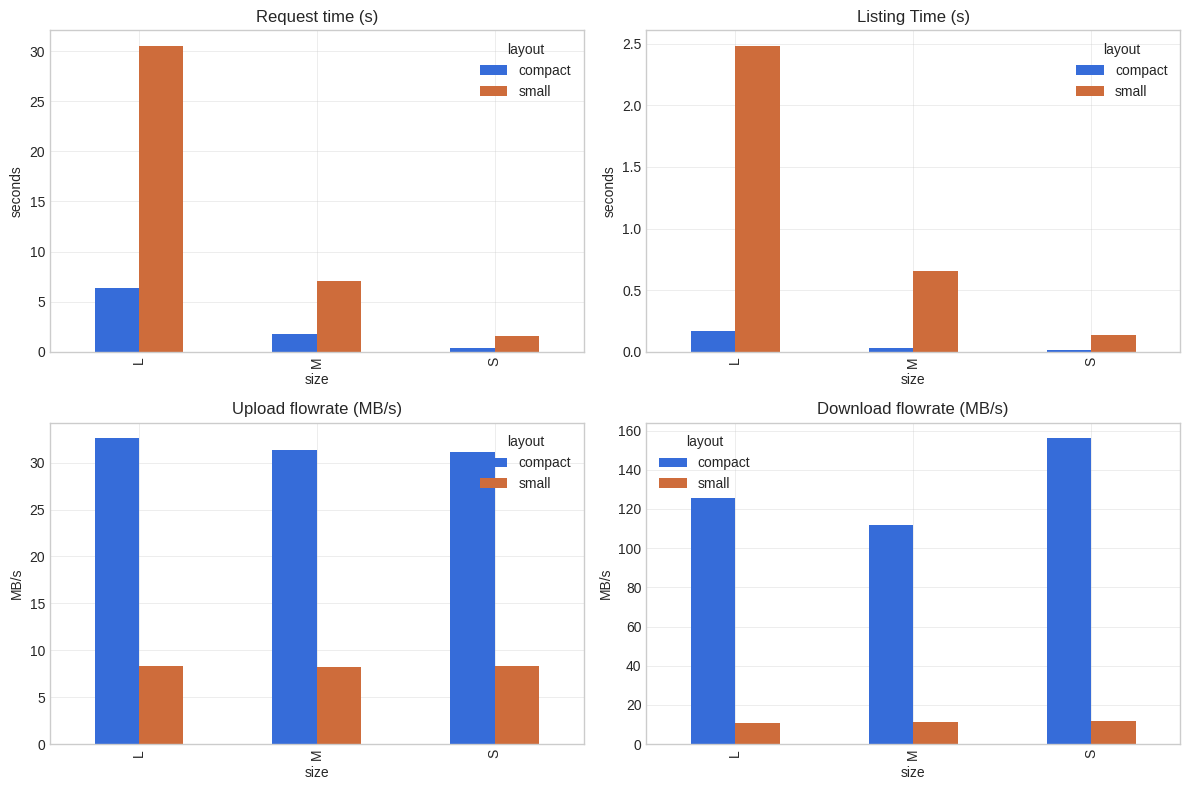
\includegraphics[width=1.25\linewidth]{output.png}%
    }
    \caption{Benchmark results for Variant 3.}
    \label{fig:variant3-results}
\end{figure}
\end{document}